\documentclass{article}
\usepackage[english]{babel}

\usepackage[a4paper,top=2cm,bottom=2cm,left=3cm,right=3cm,marginparwidth=1.75cm]{geometry}
\usepackage{amsmath}
\usepackage{unicode-math}
\usepackage{graphicx}
\usepackage[colorlinks=true, allcolors=blue]{hyperref}
\usepackage{listings}
\usepackage{minted}
\usepackage{booktabs}
\usepackage{physics}        %braket schreibweise
\setlength{\parindent}{0pt}

\title{Physics of Complex Systems: Exercise }
\author{Leopold Schaller and Daniel Lender}

\begin{document}
\maketitle

\section*{Task 4.1: Convolution product}
\subsection*{(a)}

The probability density $p(x)$ is given and its characteristic function will be calculated via

\[
\varphi(t) = E[e^{itX}]
= \int_{-\infty}^{\infty} e^{itx} p(x)\, dx.
\]

As $p(x)=0$ is valid for $x<0$, we will integrate from 0 to $\infty$.
\[
\varphi(t)
= \int_0^\infty e^{itx} w e^{-wx}\, dx = w \int_0^\infty e^{-(w - it)x}\, dx.
\]

For $\mathrm{Re}(w-it)=w>0$ and with $a = w - it$ we obtain
\[
\int_0^\infty e^{-ax}\, dx = \frac{1}{a} = \frac{1}{w - it}.
\]
Finally, we pobtain the characteristic function
\[
\boxed{
\varphi(t)
= \frac{w}{w - it}.
}
\]

\subsection*{(b) and (c)}

The two fold convolution is defined as
\[
p^{*2}_{(x)} = (p * p)(x) = \int_0^x p(y)\,p(x-y)\,dy.
\]
Higher orders are calculated by the same formula, using
\[
    (p * p * p)(x) = p^{*3}_{(x)} = (p * p^{*2}_{(x)})(x) \text{ and } p^{*N}_{(x)} = (p * p^{*N-1}_{(x)})(x)
\]

We calculate $p^{*2}_{(x)}$ explicitly and get
\[
(p * p)(x)
= \int_0^x w e^{-wy}\, w e^{-w(x-y)}\,dy = w^2 e^{-wx} \int_0^x dy = w^2 x e^{-wx}
\]
For the three fold convolution product, we get
\[
 p^{*3}_{(x)} = \int_0^x w^2 y e^{-wy} \cdot w e^{-w(x-y)} dy = w^3 e^{-wx} \int_0^x y\, dy = \frac{w^3 x^2}{2} e^{-wx} .
\]
Comparing the two solutions
\[
p^{*1}(x)=w e^{-wx}, \quad
p^{*2}(x)=w^2 x e^{-wx}, \quad
p^{*3}(x)=\frac{w^3 x^2}{2} e^{-wx}.
\]
we might observe a systematic behaviour according to
\[
p^{*N}(x)
=
\frac{w^N x^{N-1}}{(N-1)!}
e^{-wx}.
\]

because the exponential $e^y$ part will cancel out every time and what remains is an integral over a polynomial,
which increases its power by one in every convolution step.
To show this guess, we do a prove via induction:
\\
Assume that for some $N$ the formula holds:
\[
p^{*N}(x)
=
\frac{w^N x^{N-1}}{(N-1)!}
e^{-wx}.
\]

We now compute the $(N+1)$-fold convolution:
\[
p^{*(N+1)}(x)
=
\int_0^x p^{*N}(y)\, p(x-y)\, dy.
\]

Insert the induction hypothesis and $p(x)=w e^{-wx}$:
\[
=
\int_0^x \frac{w^N y^{N-1}}{(N-1)!} e^{-wy} \cdot w e^{-w(x-y)} \, dy
= \frac{w^{N+1}}{(N-1)!} e^{-wx} \int_0^x y^{N-1}\, dy.
\]

The remaining integral evaluates to
\[
\int_0^x y^{N-1}\, dy
=
\frac{x^N}{N}.
\]

Hence,
\[
p^{*(N+1)}(x)
=
\frac{w^{N+1}}{(N-1)!}
\frac{x^N}{N} e^{-wx} =
\frac{w^{N+1} x^N}{N!}
e^{-wx}.
\]

\[
p^{*(N+1)}(x)
=
\frac{w^{N+1} x^N}{N!}
e^{-wx}.
\]

This proves the formula by induction.

\subsection*{(d)}

For a one fold probability distribution $p(x) = w \, e-{-wx}$ we can calculate the expectation value and the variance to
\[
    \mu_1 = \frac{1}{w} \text{ and } \sigma_1^2 = \frac{1}{w^2}
\]
As the experiment is statistically independent, we will obtain for $p^{*(N)}(x)$
\[
    \mu_N = \frac{N}{w} \text{ and } \sigma_N^2 = \frac{N}{w^2}
\]
With $\sigma_N$ and $\mu_N$, we can built a normal distribution and compare it to the probability density $p^{*(N)}(x)$, which is shown in Fig. \ref{FigProbdis} for N = 100 and 50.
\begin{figure}[h!]
    \centering
    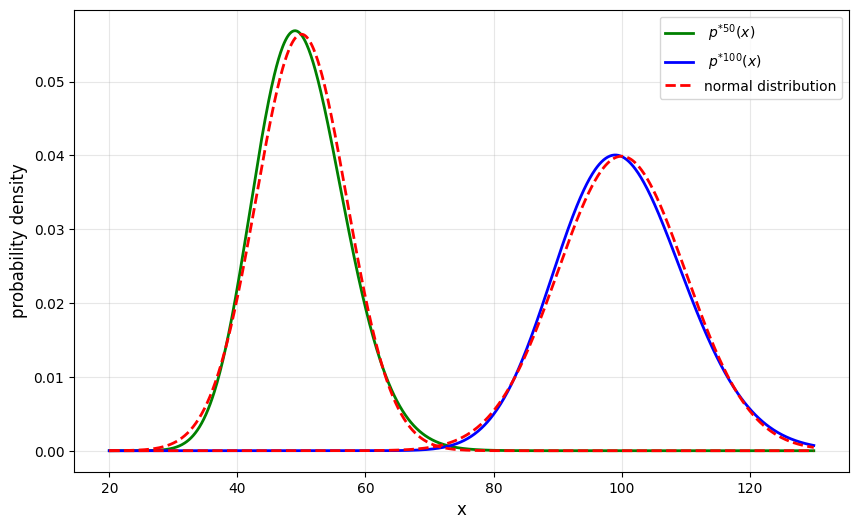
\includegraphics[width=0.9\linewidth]{Prob_distribution.png}
    \caption{Histogram for K=20 and one million generated random numbers}
    \label{FigProbdis}
\end{figure}
Both curves match very good to each other, showing the Central Limit Theorem works.

\section*{Task 4.2: Harmonic oscillator}
\subsection*{(a)}
The Liouville Operator $L_{nm}$ is defined via
\[
\frac{d}{dt} P_n(t) = \sum_m L_{nm} P_m(t),
\]
where we can insert the rates given in the sheet. We assume only transitions from n to $n\pm 1$ are possible and obtain for $n > 0$:
\[
    \frac{d}{dt} P_n(t) =  w_\uparrow P_{n-1}(t) + w_\downarrow P_{n+1}(t) - (w_\uparrow + w_\downarrow) P_{n}(t) \, ,
\]
%because the diagonal elements have to be the negative sum of each column.
As no eigenstate $\ket{-1}$ exists, the first energy level $n = 0$ is a special case:
\[
     \frac{d}{dt} P_0(t) = w_\downarrow P_{1}(t) - w_\uparrow P_{0}(t)
\]
The entire matrix reads the following:
\[
\begin{pmatrix}
- w_\uparrow &       w_\downarrow        &      0       & 0 & ... \\
  w_\uparrow & -(w_\uparrow + w_\downarrow) & w_\downarrow & 0 & ... \\
     0       &   w_\uparrow & -(w_\uparrow + w_\downarrow) & w_\downarrow & ... \\
     0       & 0 & w_\uparrow & -(w_\uparrow + w_\downarrow)  & ... \\
     0       & 0 & 0 & w_\uparrow & ... \\
     ...&...&...&...&...
\end{pmatrix}
\]

\subsection*{(b)}
The left eigenvector ist $
\mathbf{\sum} = (1, 1, 1, 1, \dots)$ and ensures that every column has a vanishing sum. The right eigenvector is calculated for the equations
\begin{align*}
    \text{n=0 : } 0 &=   w_\downarrow P_{1}(t) - w_\uparrow P_{0}(t) \Rightarrow P_1(t)=\left(\frac{\omega_\uparrow}{\omega_\downarrow}\right)P_0(t) \\
    \text{n=1 : } 0 &=  w_\uparrow P_{0}(t) + w_\downarrow P_{2}(t) - (w_\uparrow + w_\downarrow) P_{1}(t)=w_\downarrow P_{1}(t) + w_\downarrow P_{2}(t) - (w_\uparrow + w_\downarrow) P_{1}(t)\\&= w_\downarrow P_{2}(t) - w_\uparrow P_{1}(t)
    \Rightarrow P_2(t)=\left(\frac{\omega_\uparrow}{\omega_\downarrow}\right)P_1(t)=\left(\frac{\omega_\uparrow}{\omega_\downarrow}\right)^2P_0(t)
\end{align*}
now we assume for a state $n>1$:
\[
     P_{n+1}(t)=\left(\frac{\omega_\uparrow}{\omega_\downarrow}\right) P_{n}(t) \Rightarrow P_{n+1}(t)=\left(\frac{\omega_\uparrow}{\omega_\downarrow}\right)^{n+1} P_{0}(t)
\]
insert the induction hypothesis into the equation for the state $n+1$:
\begin{align*}
     0 &=  w_\uparrow P_{n}(t) + w_\downarrow P_{n+2}(t) - (w_\uparrow + w_\downarrow) P_{n+1}(t)= w_\downarrow P_{n+1}(t) + w_\downarrow P_{n+2}(t) - (w_\uparrow + w_\downarrow) P_{n+1}(t)\\
     &=w_\downarrow P_{n+2}(t) - w_\uparrow P_{n+1}(t)
    \Rightarrow P_{n+2}(t)=\left(\frac{\omega_\uparrow}{\omega_\downarrow}\right)P_{n+1}(t)=\left(\frac{\omega_\uparrow}{\omega_\downarrow}\right)^2P_n(t)\\
    \Rightarrow P_{n+2}&=\left(\frac{\omega_\uparrow}{\omega_\downarrow}\right)^{n+2} P_0(t)
\end{align*}
Now we proved 
\[
    P_n = \left(  \frac{w_\uparrow}{w_\downarrow} \right)^n P_0
\]
by induction. Where $P_n$ is the n-th component of the right eigenvector to the eigenvalue zero.
\subsection*{(c)}
The normalization condition yields :
\begin{align*}
    1 &= \mathbf{\sum} \cdot \vec{P_n} = \sum_{n=0}^{\infty}  P_n = P_0 \sum_{n=0}^{\infty} \left(\frac{w_\uparrow}{w_\downarrow}\right)^n = P_0  \left(\frac{1}{1-\frac{w_\uparrow}{w_\downarrow}}\right) \\
       \Rightarrow P_0 &= 1-\frac{w_\uparrow}{w_\downarrow}\\
\end{align*}
The calculation contains a geometric series, it only converges, if the condition $w_\uparrow < w_\downarrow$ is fulfilled.

Now we can express the components of the right eigenvector to the eigenvalue zero only dependent from $\omega_\uparrow$ and $\omega_\downarrow$:
\begin{align*}
    P_n= \left(1-\frac{\omega_\uparrow}{\omega_\downarrow}\right)\left(\frac{\omega_\uparrow}{\omega_\downarrow}\right)^n= \left(\frac{\omega_\uparrow}{\omega_\downarrow}\right)^n-\left(\frac{\omega_\uparrow}{\omega_\downarrow}\right)^{n+1}
\end{align*}

\subsection*{(d)}
The probability distribution in a canonical ensemble is 
\begin{align*}
    p_n \propto \text{exp}\left(\frac{E_n}{k_B T}\right) &= \text{exp}\left(\frac{\hbar \omega }{2k_B T}\right)\cdot \text{exp}\left(\frac{\hbar \omega n}{k_B T}\right)\\
    &=A\cdot \left[\text{exp}\left(\frac{\hbar \omega}{k_B T}\right)\right]^n
\end{align*}
Furthermore we know
\begin{align*}
    p_n\propto\left(\frac{\omega_\uparrow}{\omega_\downarrow}\right)^n
\end{align*}
Comparing the base of the exponent for both terms leads to this expression: 
\begin{align}
        \frac{w_\uparrow}{w_\downarrow} &= e^{\frac{\hbar \omega}{k_B T}}\\
        \Rightarrow \text{ln}\left(\frac{\omega_\uparrow}{\omega_\downarrow}\right)&=-\frac{\hbar\omega}{k_BT}
\end{align}
solving for T yields
\begin{align}
    T = -\frac{\hbar \omega}{k_B \text{ln}\left({\frac{w_\uparrow}{w_\downarrow}}\right)}=\frac{\hbar \omega}{k_B \text{ln}\left({\frac{w_\downarrow}{w_\uparrow}}\right)}
\end{align}
\end{document}


# latexmk -pdf -shell-escape -output-directory=out Uebung4/exercise4/exercise4_Schaller_Lender.tex


